\subsection{Edge}

\subsubsection{Descripción}

\begin{multicols}{2}
El filtro EDGE devuelve una imagen con los bordes de otra imagen original. Esto se logra observando los píxeles donde la intensidad de la imagen cambia de forma abrupta. A su vez esto puede ser logrado buscando saltos en una función de intensidades. Esta idea de detectar los bordes fue implementada a través del operador de Laplace, cuya matriz es: 

$$ M = \left(
\begin{matrix}
    0.5 & 1 & 0.5 \\
    1 & -6 & 1 \\
    0.5 & 1 & 0.5
\end{matrix}
\right)$$

\begin{center}
	\begin{tabular}{cccc}
		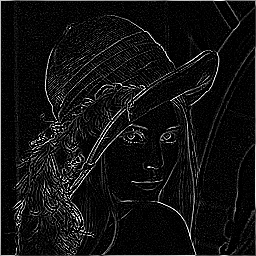
\includegraphics[width=0.3\textwidth]{imagenes/lenaEDGA.jpg} \\
		\end{tabular}
	\end{center}
\end{multicols}

La forma de utilizarla es posicionando uno a uno cada píxel en el centro de la matriz y realizando el siguiente cálculo: 

$$dst(x, y) = \sum_{k = 0}^2 \sum_{l = 0}^2 src(x + k - 1, y + l - 1) * M(k, l)$$

Al igual que monocromatizar, EDGE opera sobre imágenes en escala de grises (1 componente de color por píxel). Como no se pueden procesar los bordes con la función anterior se aplica la siguiente función: $dst(x, y) = src(x,y)$.

\subsubsection{Implementación C}

Ignorando la primera y la última fila al igual que el primer y el último pixel de cada fila, recorrimos iterativamente todos los píxeles de la imagen realizando el siguiente proceso: por cada pixel calculamos todas las sumas parciales de la función que resulta de la aplicación de la matriz de Laplace, luego todas estas sumas fueron almacenadas en una variable auxiliar (\textit{edge}). Si el valor de \textit{edge} requería ser saturado se lo restringió a los valores 0/255 y finalmente se guardó el resultado en el píxel correspondiente de la imagen destino.

\begin{algorithm}[H]
  \begin{algorithmic}[1]
		\FORALL{y:=1 \TO  Height($I_{src}$$-1$)}
			\FORALL{x:=1 \TO  Width($I_{src}$)$-1$}
			  \STATE $m_{0,0} \gets I_{src}(x-1,y-1)*0.5$
			  \STATE $m_{0,1} \gets I_{src}(x-1,y)*1$
			  \STATE $m_{0,2} \gets I_{src}(x-1,y+1)*0.5$
			  \STATE $m_{1,0} \gets I_{src}(x,y-1)*1$
			  \STATE $m_{1,1} \gets I_{src}(x,y)*(-6)$
			  \STATE $m_{1,2} \gets I_{src}(x,y+1)*1$
			  \STATE $m_{2,0} \gets I_{src}(x+1,y-1)*0.5$
			  \STATE $m_{2,1} \gets I_{src}(x+1,y)*1$
			  \STATE $m_{2,2} \gets I_{src}(x+1,y+1)*0.5$
			  \STATE $edge \gets m_{0,0}+m_{0,1}+m_{0,2}+m_{1,0}+m_{1,1}+m_{1,2}+m_{2,0}+m_{2,1}+m_{2,2}$
			  \STATE $I_{dst}(x,y) \gets Saturar(edge)$
			\ENDFOR
		 \ENDFOR
  \end{algorithmic}
  \caption{$edge (I_{src}, I_{dst})$}
  \label{alg:edge}
\end{algorithm}

\subsubsection{Implementación ASM}

Como previamente habíamos comentado, copiaremos los píxeles del borde tal como estaban en la imagen original. Sabiendo eso explicaremos las partes más relevantes de los cálculos realizados con las intrucciones de assembler.

\subsubsection*{Obtenemos la matriz de píxeles}

\begin{multicols}{2}
En este filtro procesaremos de a 2 componentes por cada píxel. Brindamos un dibujo de como se ve la imagen en memoria y donde apuntan los registros(punteros). En este caso \emph{rdi} apunta al píxel con el que vamos a trabajar, y \emph{rdx} contiene el ancho de la imagen. Por otro lado la \emph{matriz} muestra como ven los registros \emph{xmm}a los pixeles. Tenemos la parte  \emph{alta, centro y baja}, como se muestra en la matriz para procesar la imagen.
\begin{center}
		$rdi \gets PunteroAPixel$ \\
		$rdx \ width$
\end{center}

\begin{center}
\[ \left( \begin{array}{cccc}
 a_0 & b_0 & g_0 & r_0 \\ 
 a_1 & b_1 & g_1 & r_1 \\
 a_2 & b_2 & g_2 & r_2
\end{array} \right) = \left( \begin{array}{cccc}
 Pixel_1 \\ 
 Pixel_2 \\
 Pexel_3
\end{array} \right)\ = \left( \begin{array}{cccc}
 Alta \\ 
 Centro \\
 Baja
\end{array} \right)\] 

\end{center}

    \begin{center}
	    \begin{tabular}{cccc}
		  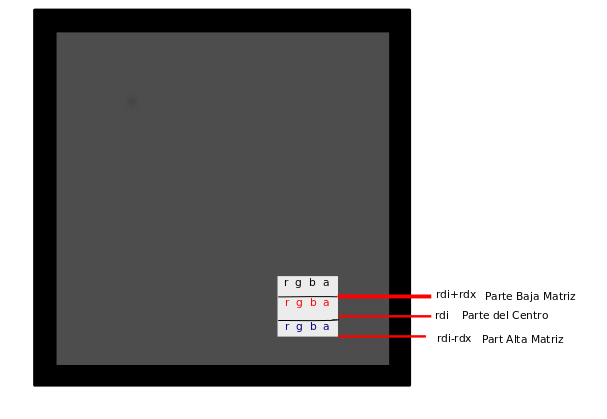
\includegraphics[width=0.6\textwidth]{imagenes/edge/edge1.png} \\
		\end{tabular}
	\end{center}

\end{multicols}

\begin{codesnippet}
\begin{verbatim}    
;Obtenemos el píxel de la imagen fuente en eax
    mov eax, [rdi]          ;eax=|a b g r|

                            ;Caso centro de la matriz
    pxor xmm2, xmm2         ;xmm2=|0 0 0 0|
    pxor xmm1, xmm1         ;xmm1=|0 0 0 0|
    pxor xmm0, xmm0         ;xmm0=|0 0 0 0|
    movd xmm0, eax          ;xmm0=|0|0|0|a b g r|
    punpcklbw xmm0, xmm1    ;xmm0=|0|a b g r| convert de byte a word parte baja
    movd xmm1, eax          ;xmm1=|0|0|0|a b g r|
    punpcklbw xmm1, xmm2    ;xmm1=|0|a b g r|     
    pslldq xmm0, 8          ;xmm0=|a b g r|0|
    paddw xmm0, xmm1        ;xmm0=|a b g r|a b g r| centro de la matriz

;Caso Parte baja de la matriz, son los mismos cálculos, solo cambia el puntero a la imagen.

    mov eax, [rdi + rdx]    ;eax=|a b g r| observar rdi+rdx donde rdx= width
    paddw xmm1, xmm2        ;xmm1=|a b g r|a b g r| Baja: parte baja de la matriz

;Caso Parte Alta es análoga

    mov eax, [rdi + r9]     ;mov eax,[rdi-width]
    paddw xmm2, xmm3        ;xmm2=|a b g r|a b g r| Alta: parte alta de la matriz	
\end{verbatim}
\end{codesnippet}

\subsubsection*{Armado y multiplicación de la matriz}

En esta sección hacemos la multiplicación anteriormente mencionada en el enunciado.

\begin{codesnippet}
\begin{verbatim}    
                                   ;dividimos por 2 a xmm2 y xmm1
    psrlw xmm2, 1                  ;xmm2=|a/2 b/2 g/2 r/2|a/2 b/2 g/2 r/2| Matriz Alta
    psrlw xmm1, 1                  ;xmm1=|a/2 b/2 g/2 r/2|a/2 b/2 g/2 r/2| Matriz Baja

                                   ;xmm0=|a b g r|a b g r| Centro
    pshuflw xmm0, xmm0, 10010000b  ;xmm0=|a b g r|b g r r| shift word parte baja [63:0]
    pshufhw xmm0, xmm0, 11100101b  ;xmm0=|a b g g|b g r r| shift word parte alta [127:64]

                                   ;xmm1=|a/2 b/2 g/2 r|a/2 b/2 g/2 r/2| Baja
    pshuflw xmm1, xmm1, 10010000b  ;xmm1=|a/2 b/2 g/2 r/2|b/2 g/2 r/2 r/2| 
    pshufhw xmm1, xmm1, 11100101b  ;xmm1=|a/2 b/2 g/2 g/2|b/2 g/2 r/2 r/2|

                                   ;xmm2=|a/2 b/2 g/2 r/2|a/2 b/2 g/2 r/2| Alta
    pshuflw xmm2, xmm2, 10010000b  ;xmm2=|a/2 b/2 g/2 r/2|b/2 g/2 r/2 r/2|
    pshufhw xmm2, xmm2, 11100101b  ;xmm2=|a/2 b/2 g/2 g/2|b/2 g/2 r/2 r/2|
                                   ;shiftea cada paquete quad word a derecha cant de bits
    psrlq xmm0, 16                 ;xmm0=|0 a b g|0 b g r| Centro
    psrlq xmm1, 16                 ;xmm1=|0 a/2 b/2 g/2|0 b/2 g/2 r/2| BAja
    psrlq xmm2, 16                 ;xmm2=|0 a/2 b/2 g/2|0 b/2 g/2 r/2| Alta
                                   ;shiftea cada paquete quad word a izquierda cantidad de bit

    psllq xmm2, 16                 ;xmm2=|a/2 b/2 g/2 0|b/2 g/2 r/2 0| Alta
    psllq xmm0, 16                 ;xmm0=|a    b   g  0|b   g   r   0| Centro
    psllq xmm1, 16                 ;xmm1=|a/2 b/2 g/2 0|b/2 g/2 r/2 0| Baja
\end{verbatim}
\end{codesnippet}

\begin{codesnippet}
\begin{verbatim}    
								   ;Armamos la Matriz
                                   ;multiplicamos xmm2 por los valores de la matriz
                                   ;xmm14=|1 2 1 1|1 2 1 1|
                                   ;xmm15=|1 -6 1 1|1 -6 1 1|
    pmullw xmm2, xmm14             ;xmm2=|a/2 b g/2 0|b/2 g r/2 0| Alta
    pmullw xmm0, xmm15			   ;xmm0=|a -6*b g  0 |b -6*g r 0| Centro
    pmullw xmm1, xmm14			   ;xmm1=|a/2 b g/2 0|b/2 g r/2 0| Baja
\end{verbatim}
\end{codesnippet}

Una vez que tenemos armada la matriz. Solamente hace falta sumarlas, para eso aplicamos sumas verticales y luego sumas horizontales como podemos ver a continuación:

\begin{codesnippet}
\begin{verbatim}    
    paddw xmm1, xmm2                ;xmm1=|a/2+a/2 b+b g/2*g/2 0|b/2+b/2 g+g r/2*r/2 0| Baja+Alta
    paddw xmm0, xmm1                ;xmm0=|a+a/2+a/2 -6*b+b+b g+g/2*g/2 0| 
                                    ;     |b+b/2+b/2 -6*g+g+g r+r/2*r/2 0| Centro + Baja + Alta	

                                    ;Suma horizontal
                                    ;xmm0=|s7 s6 s5 s4| s3 s2 s1 s0|
    phaddw xmm0, xmm0               ;xmm0=|s7+s6 s5+s4 s3+s2 s1+s0|s7+s6 s5+s4 s3+s2 s1+s0|
    phaddw xmm0, xmm0               ;xmm0=|s7+s6+s5+s4 s3+s2+s1+s0 s7+s6+s5+s4 s3+s2+s1+s0|
                                    ;     |s7+s6+s5+s4 s3+s2+s1+s0 s7+s6+s5+s4 s3+s2+s1+s0|  
                                    ;xmm0=|s[7:4]s[3:0]s[7:4]s[3:0]|s[7:4]s[3:0]s[7:4]s[3:0]|
                                    ;xmm0=|. . . .|. . s[7:4] s[3:0]|
\end{verbatim}
\end{codesnippet}

Y como último paso resta copiar a memoria \emph{xmm0}, para eso usamos instrucciones de \emph{shift} y \emph{movq}. Todos estos pasos se repiten para toda la imagen, exceptuando los bordes.